\section{Testování výkonu objektových databází}
V této podkapitole se pustím do samotného testování objektových databází. Mezi testované databáze, které jsem pro účel své práce zvolil. Patří databáze DB4O, OrientDB a ObjectDB. Důvodem výběru těchto tří, byla dostupnost zdarma a aktivní vývoj (na obrázku \ref{img:oodbms:comp} je přehled jejich vlastností). ObjectDB je sice komerční databáze, ale pro omezené potřeby (max 10 entitních tříd a 1 milión instancí entit) je možně ji využívat zcela bez poplatků.

Výsledky jednotlivých testů vidíme na obrázcích \ref{img:oodbms1} až \ref{img:oodbms14}.

\begin{figure}[!h]
  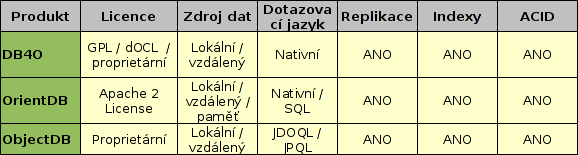
\includegraphics[width=38em]{obr/oodbms_comp}
  \caption{Přehled vlastností}\label{img:oodbms:comp}
\end{figure}

\section{Testování výkonu objektově relačního mapování }
V této podkapitole se pustím do samotného testování JPA (ORM) frameworků. Mezi testované JPA implementace jsem zařadil Hibernate, EclipseLink,OpenJPA, DataNucleus a BatooJPA (přehled základních vlastností a informací je na obrázku \ref{img:jpa:comp}). Jednotlivé výsledky testů vidíme na obrázcích \ref{img:jpa1} až \ref{img:jpa14}.
\begin{figure}[!h]
  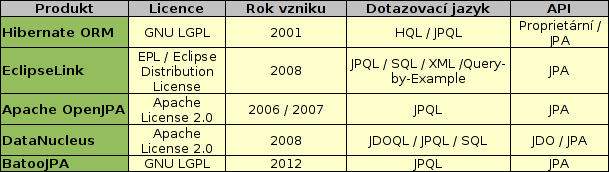
\includegraphics[width=38em]{obr/jpa_comp}
  \caption{Přehled vlastností}\label{img:jpa:comp}
\end{figure}
\begin{figure}[!h]
  \begin{subfigure}[b]{0.5\textwidth}
  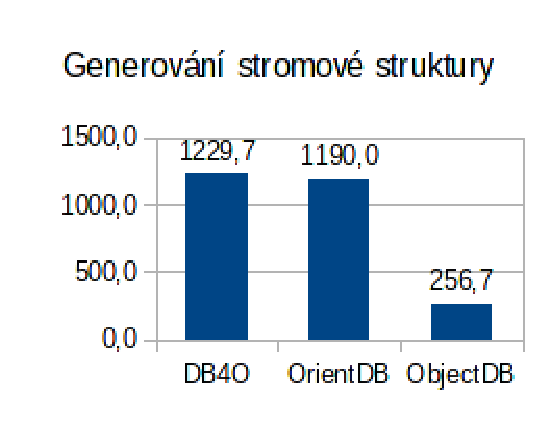
\includegraphics[]{obr/bench/oodbms1}
  \caption{Generování stromové struktury [ms]}\label{img:oodbms1}
  \end{subfigure}
  \begin{subfigure}[b]{0.5\textwidth}
  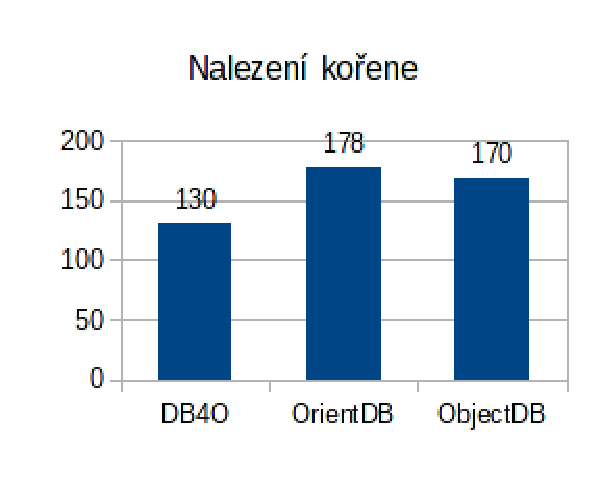
\includegraphics[]{obr/bench/oodbms2}
  \caption{Nalezení kořene [ms]}\label{img:oodbms2}
  \end{subfigure}
  \begin{subfigure}[b]{0.5\textwidth}
  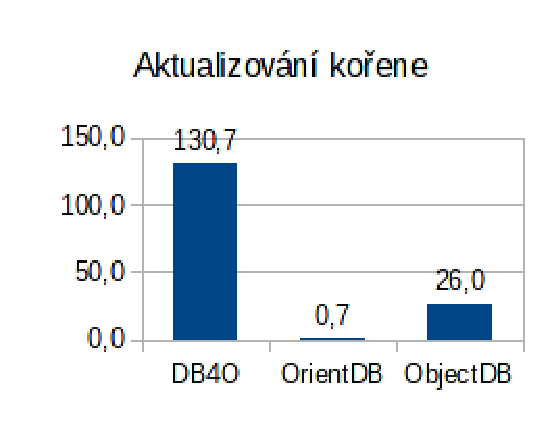
\includegraphics[]{obr/bench/oodbms3}
  \caption{Aktualizování kořene [ms]}\label{img:oodbms3}
  \end{subfigure}
  \begin{subfigure}[b]{0.5\textwidth}
  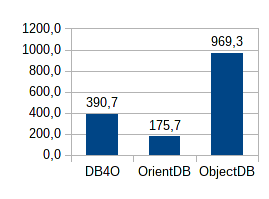
\includegraphics[]{obr/bench/oodbms4}
  \caption{Nalezení listů [ms]}\label{img:oodbms4}
  \end{subfigure}
  \begin{subfigure}[b]{0.5\textwidth}
  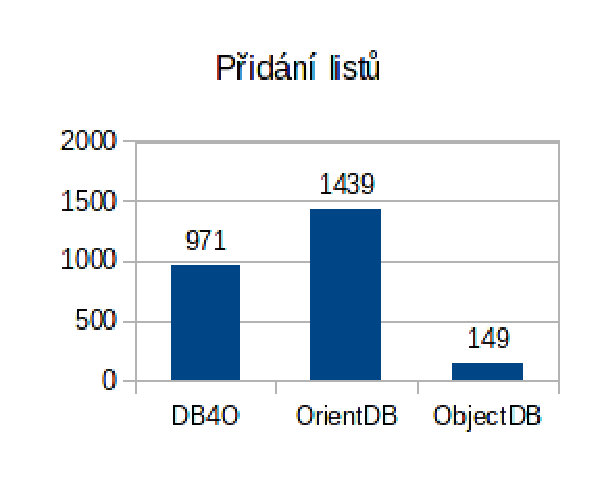
\includegraphics[width=18em]{obr/bench/oodbms5}
  \caption{Přidání listů [ms]}\label{img:oodbms5}
  \end{subfigure}
  \begin{subfigure}[b]{0.5\textwidth}
  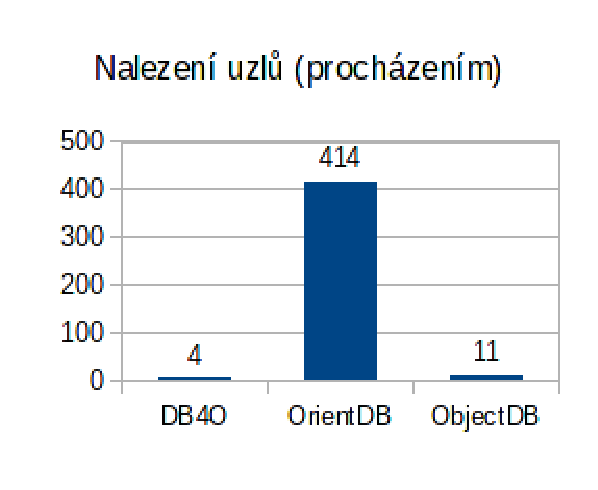
\includegraphics[]{obr/bench/oodbms6}
  \caption{Nalezení uzlů (procházením) [ms]}\label{img:oodbms6}
  \end{subfigure}
  \begin{subfigure}[b]{0.5\textwidth}
  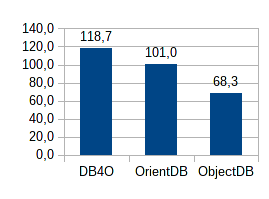
\includegraphics[]{obr/bench/oodbms7}
  \caption{Nalezení uzlů (dotazem) [ms]}\label{img:oodbms7}
  \end{subfigure}
  \begin{subfigure}[b]{0.5\textwidth}
  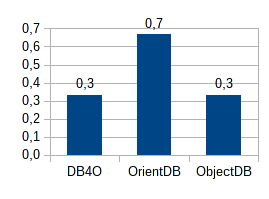
\includegraphics[]{obr/bench/oodbms8}
  \caption{Průchod stromem [ms]}\label{img:oodbms8}
  \end{subfigure}
\end{figure}
\begin{figure}[!h]\ContinuedFloat
  \begin{subfigure}[b]{0.5\textwidth}
  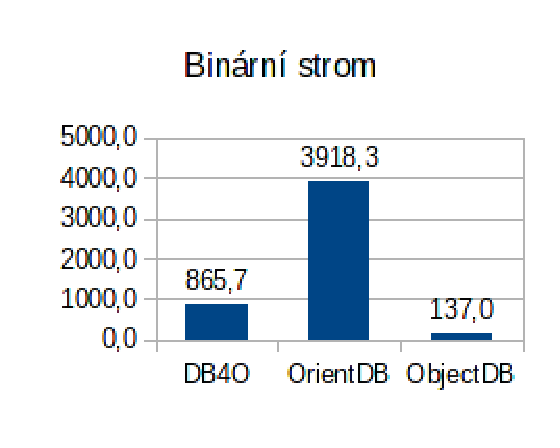
\includegraphics[]{obr/bench/oodbms9}
  \caption{Binární strom [ms]}\label{img:oodbms9}
  \end{subfigure}
  \begin{subfigure}[b]{0.5\textwidth}
  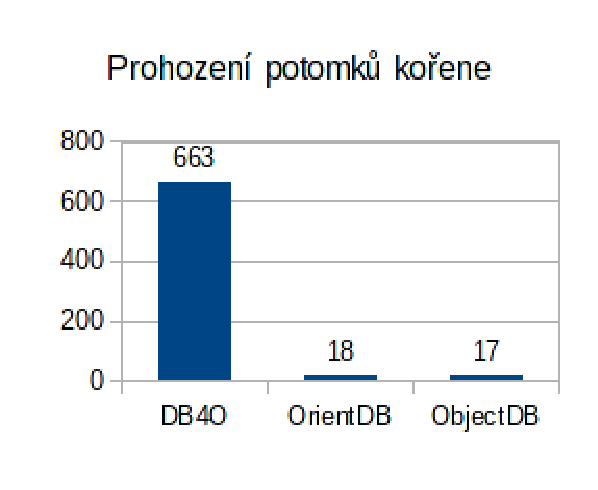
\includegraphics[]{obr/bench/oodbms10}
  \caption{Prohození potomků kořene [ms]}\label{img:oodbms10}
  \end{subfigure}
  \begin{subfigure}[b]{0.5\textwidth}
  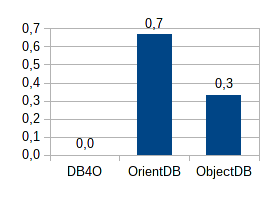
\includegraphics[]{obr/bench/oodbms11}
  \caption{Průchod binárním stromem [ms]}\label{img:oodbms11}
  \end{subfigure}
  \begin{subfigure}[b]{0.5\textwidth}
  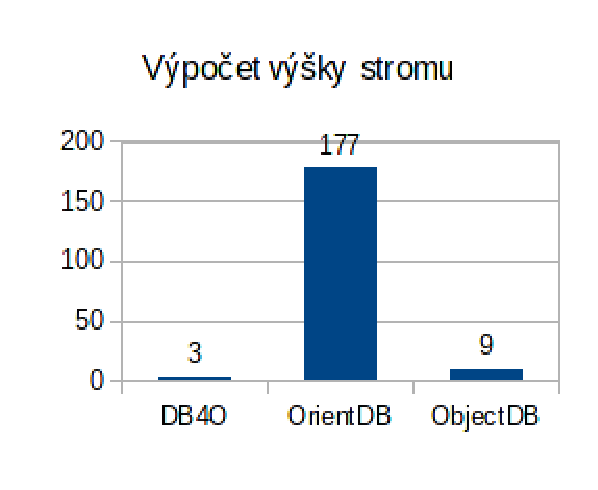
\includegraphics[]{obr/bench/oodbms12}
  \caption{Výpočet výšky stromu [ms]}\label{img:oodbms12}
  \end{subfigure}
  \begin{subfigure}[b]{0.5\textwidth}
  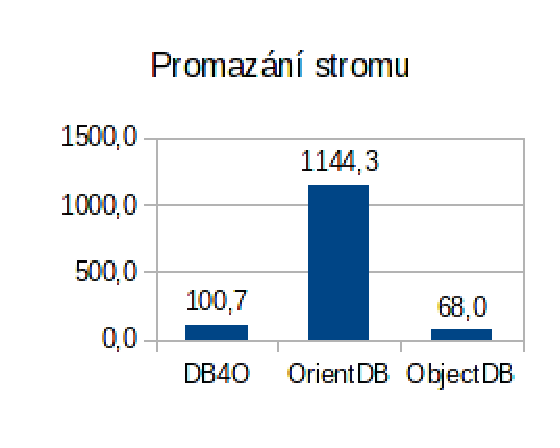
\includegraphics[]{obr/bench/oodbms13}
  \caption{Promazání stromu [ms]}\label{img:oodbms13}
  \end{subfigure}
  \begin{subfigure}[b]{0.5\textwidth}
  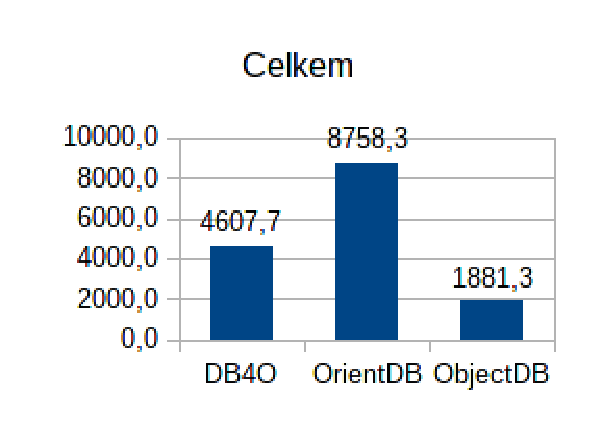
\includegraphics[]{obr/bench/oodbms14}
  \caption{Celkový čas [ms]}\label{img:oodbms14}
  \end{subfigure}
\end{figure}

